\documentclass[aspectratio=169]{beamer}
\usepackage[T1]{fontenc}
\usepackage[utf8]{inputenc}
\usepackage{listings}
\usepackage{colortbl}
\usepackage{tikz}
\usetikzlibrary{positioning,fit,calc,arrows.meta}
\usepackage[scaled=.92]{helvet}
%\renewcommand*\sfdefault{cmss}
%\usepackage[sfmath]{kpfonts}

\definecolor{codegreen}{rgb}{0,0.6,0}
\definecolor{codegray}{rgb}{0.5,0.5,0.5}
\definecolor{codepurple}{rgb}{0.58,0,0.82}
\definecolor{backcolour}{rgb}{0.95,0.95,0.92}

\lstdefinestyle{mystyle}{
    backgroundcolor=\color{backcolour},
    commentstyle=\color{codegreen},
    keywordstyle=\color{magenta},
    numberstyle=\tiny\color{codegray},
    stringstyle=\color{codepurple},
    basicstyle=\ttfamily\footnotesize,
    breakatwhitespace=false,
    breaklines=true,
    captionpos=b,
    keepspaces=true,
    numbers=left,
    numbersep=5pt,
    showspaces=false,
    showstringspaces=false,
    showtabs=false,
    tabsize=2
}

\lstset{style=mystyle}

\title{Leveraging Local LLMs for\\Automated Changelog Generation}
\author{Christian Goll <\texttt{cgoll@suse.com}>}
\date{\today}
\usetheme{suse}

\begin{document}
\begin{frame}
  \titlepage
\end{frame}

% \begin{frame}{Outline}
%   \tableofcontents
% \end{frame}

\begin{frame}[fragile]{Quickstart}
\begin{block}{Tumbelweed}
\begin{lstlisting}[language=bash, basicstyle=\ttfamily\tiny]
#> sudo zypper in python-changelog-gen
#> cd SUPER_DUPER_PKG
#> osc-ai-vc
\end{lstlisting}
\end{block}
\begin{block}{Leap 16.0}
\begin{lstlisting}[language=bash, basicstyle=\ttfamily\tiny]
#> sudo zypper ar obs://science:machinelearning sc:ml
#> sudo zypper in python-changelog-gen
#> cd SUPER_DUPER_PKG
#> osc-ai-vc
\end{lstlisting}
\end{block}
\begin{block}{Resources}
\url{https://huggingface.co/mslacken/t5-finetune-changelog}\\
\url{https://github.com/openSUSE/changelog-gen}
\end{block}
\end{frame}

\section{Introduction}
\begin{frame}{Motivation}
  \begin{block}{Changelogs in Open Build Service}
    \begin{itemize}
      \item Changelog of packages are created from \texttt{.changes} file
      \item Mostly reflect upstream changelog
      \item \textbf{But} must also contain changes for package creation
    \end{itemize}
  \end{block}
  \begin{block}{The Opportunity}
    \begin{itemize}
      \item Accepted requests to \texttt{openSUSE:Factory} should all be in the right format
      \item submission requests contain the necessary information
      \item Perfect candidate for LLM automation
    \end{itemize}
  \end{block}
\end{frame}

\begin{frame}{Why Fine-tune a Local LLM?}
\begin{columns}
\column{0.6\textwidth}
\begin{block}{Existing tools}
\begin{itemize}
  \item Existing tools can the same
  \item Can't pickup changes to \texttt {.spec} or \texttt{\_multibuild} files
\end{itemize}
\end{block}
\begin{block}{Advantages}
\begin{itemize}
  \item \textbf{Hype Train}
  \item pickup semantic changes like avoid to mention changes regarding Apple
  \item possible to run complete locally, can handle embargoed changes
\end{itemize}
\end{block}
\column{0.3\textwidth}
  
\includegraphics[width=\linewidth]{Thought Train}
\end{columns}
\end{frame}

\section{T5 model}
\begin{frame}{Which model to choose}
\begin{columns}
\column{0.6\textwidth}
\begin{block}{Constraints}
\begin{itemize}
    \item model must be small (arround $1\texttt{Gb}$)
    \item permissive license
    \item not quantized, so that it can be finetuned
    \item transformer based and no GPT model
\end{itemize}
\end{block}
\column{0.3\textwidth}
  
\includegraphics[width=\linewidth]{Thinking Chameleon}
\end{columns}
\end{frame}

\begin{frame}{Encoder-Decoder vs Decoder-Only}
\begin{block}{Encoder-Decoder: T5, BART, mT5}
\begin{itemize}
  \item \textbf{Bidirectional encoder}: Sees entire input at once
  \item Best for: Translation, summarization, structured text generation
\end{itemize}
\end{block}

\begin{block}{Decoder-Only: GPT-3, GPT-4, LLaMA, Mistral}
\begin{itemize}
  \item \textbf{Single decoder}: Input and output in same stream but only sees previous tokens
  \item Best for: Text completion, general-purpose chat
\end{itemize}
\end{block}

\begin{alertblock}{Key Difference}
T5 can \textbf{read all input first}, then generate. GPT processes input and output sequentially. This makes T5 more efficient for tasks with structured input.
\end{alertblock}
\end{frame}

\begin{frame}{Encoder-Decoder Architecture (T5)}
\begin{columns}
\column{0.4\textwidth}
\begin{itemize}
    \item \textbf{Encoder}: Bidirectional processing of the input sequence.
    \item \textbf{Decoder}: Autoregressive generation with cross-attention to encoder.
\end{itemize}
\column{0.6\textwidth}
\centering
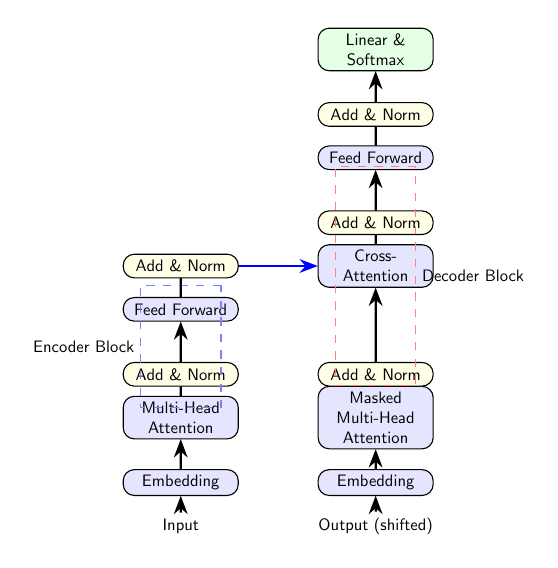
\begin{tikzpicture}[scale=0.55, every node/.style={scale=0.6, font=\sffamily}]
    \tikzset{block/.style={rectangle, draw, fill=blue!10, text width=2.2cm, text centered, rounded corners, minimum height=0.5cm}}
    \tikzset{norm/.style={rectangle, draw, fill=yellow!10, text width=2.2cm, text centered, rounded corners, minimum height=0.5cm}}
    \tikzset{line/.style={draw, -{Stealth[scale=1.0]}, thick}}

    % Encoder
    \node (e_in) at (0,0) {Input};
    \node [block] (e_emb) at (0,1) {Embedding};
    \node [block] (e_att) at (0,2.5) {Multi-Head Attention};
    \node [norm] (e_n1) at (0,3.5) {Add \& Norm};
    \node [block] (e_ff) at (0,5) {Feed Forward};
    \node [norm] (e_n2) at (0,6) {Add \& Norm};
    \node [fit=(e_att) (e_n2), draw, blue!50, dashed, label=left:Encoder Block] {};

    % Decoder
    \node (d_in) at (4.5,0) {Output (shifted)};
    \node [block] (d_emb) at (4.5,1) {Embedding};
    \node [block] (d_att_m) at (4.5,2.5) {Masked Multi-Head Attention};
    \node [norm] (d_n1) at (4.5,3.5) {Add \& Norm};
    \node [block] (d_att_c) at (4.5,6) {Cross-Attention};
    \node [norm] (d_n2) at (4.5,7) {Add \& Norm};
    \node [block] (d_ff) at (4.5,8.5) {Feed Forward};
    \node [norm] (d_n3) at (4.5,9.5) {Add \& Norm};
    \node [fit=(d_att_m) (d_n3), draw, red!50, dashed, label=right:Decoder Block] {};

    \node [block, fill=green!10] (out) at (4.5,11) {Linear \& Softmax};

    \path [line] (e_in) -- (e_emb);
    \path [line] (e_emb) -- (e_att);
    \draw [thick] (e_att) -- (e_n1);
    \path [line] (e_n1) -- (e_ff);
    \draw [thick] (e_ff) -- (e_n2);

    \path [line] (d_in) -- (d_emb);
    \path [line] (d_emb) -- (d_att_m);
    \draw [thick] (d_att_m) -- (d_n1);
    \path [line] (d_n1) -- (d_att_c);
    \draw [thick] (d_att_c) -- (d_n2);
    \path [line] (d_n2) -- (d_ff);
    \draw [thick] (d_ff) -- (d_n3);
    \path [line] (d_n3) -- (out);

    \draw [line, blue] (e_n2.east) -- (d_att_c.west);
\end{tikzpicture}
\end{columns}
\end{frame}

\begin{frame}{Decoder-Only Architecture (GPT/LLaMA)}
\begin{columns}
\column{0.4\textwidth}
\begin{itemize}
    \item \textbf{Streamlined}: Unified architecture for both input and output.
    \item \textbf{Causal Masking}: Each token only attends to previous tokens.
\end{itemize}
\column{0.6\textwidth}
\centering
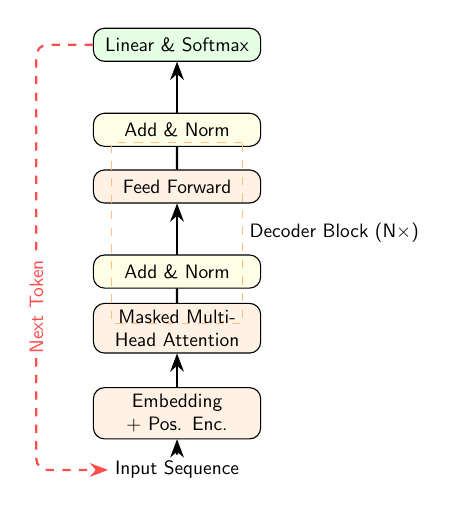
\begin{tikzpicture}[scale=0.6, every node/.style={scale=0.7, font=\sffamily}]
    \tikzset{block/.style={rectangle, draw, fill=orange!10, text width=2.8cm, text centered, rounded corners, minimum height=0.6cm}}
    \tikzset{norm/.style={rectangle, draw, fill=yellow!10, text width=2.8cm, text centered, rounded corners, minimum height=0.6cm}}
    \tikzset{line/.style={draw, -{Stealth[scale=1.0]}, thick}}

    \node (in) at (0,0) {Input Sequence};
    \node [block] (emb) at (0,1.2) {Embedding + Pos. Enc.};
    \node [block] (att) at (0,3) {Masked Multi-Head Attention};
    \node [norm] (n1) at (0,4.2) {Add \& Norm};
    \node [block] (ff) at (0,6) {Feed Forward};
    \node [norm] (n2) at (0,7.2) {Add \& Norm};
    \node [fit=(att) (n2), draw, orange!50, dashed, label=right:Decoder Block (N$\times$)] {};

    \node [block, fill=green!10] (out) at (0,9) {Linear \& Softmax};

    \path [line] (in) -- (emb);
    \path [line] (emb) -- (att);
    \draw [thick] (att) -- (n1);
    \path [line] (n1) -- (ff);
    \draw [thick] (ff) -- (n2);
    \path [line] (n2) -- (out);

    \draw [line, rounded corners, dashed, red!70, -{Stealth[scale=1.0]}] (out.west) -- ++(-1.2,0) |- (in.west) node[pos=0.25, left, rotate=90, fill=white, inner sep=1pt] {Next Token};
\end{tikzpicture}
\end{columns}
\end{frame}
\begin{frame}{T5: Origins and History}
\begin{block}{The T5 Paper (2019) by Google}
\begin{itemize}
  \item \textbf{T5 = Text-To-Text Transfer Transformer}
  \item Systematic study of NLP transfer learning
  \item \textbf{Everything is text-to-text}
  \item Apache 2.0 License
\end{itemize}

\end{block}
\begin{block}{Pre-training}
\begin{itemize}
  \item Trained on C4 dataset (Colossal Clean Crawled Corpus)
  \item 750 GB of cleaned web text
\end{itemize}
\end{block}
\end{frame}

\begin{frame}{T5 Architecture: Encoder-Decoder}
\begin{columns}[t]
\column{0.5\textwidth}
\begin{block}{Encoder-Decoder Design}
\begin{itemize}
  \item \textbf{Encoder}: Processes input text
  \begin{itemize}
    \item Bidirectional attention
    \item Understands full context
    \item Creates rich representations
  \end{itemize}
  \item \textbf{Decoder}: Generates output text
  \begin{itemize}
    \item Autoregressive generation
    \item Attends to encoder outputs
    \item Produces token-by-token
  \end{itemize}
\end{itemize}
\end{block}
\column{0.5\textwidth}

\begin{block}{Model Sizes}
\centering
\vspace{0.5cm}
\begin{tabular}{lrrr}
\hline
\textbf{Model} & \textbf{Params} & \textbf{Layers} & \textbf{Size} \\ \hline
Small & 60M  & 12 & 242 MB \\
Base  & 220M & 24 & 892 MB \\
Large & 770M & 48 & 2.75 GB \\ \hline
\end{tabular}
\end{block}
\vfill
\end{columns}
\end{frame}

\section{Data Collection Pipeline}
\begin{frame}[fragile]{OBS Data Extraction}
\begin{block}{What data do we need?}
\begin{itemize}
  \item Accepted requests to \texttt{openSUSE:Factory}
  \item Spec file diffs (version updates, build changes)
  \item Source file changes (added, removed, modified)
  \item Release notes from upstream (GitHub, archive changelogs)
  \item The actual \texttt{.changes} file entries (our target)
\end{itemize}
\end{block}
\end{frame}
\end{document}

